\section{Performance Analysis}
%4.1) Balancing between two paths with high loss using fixed time unit
% using only loss-based balance in a simple regime where that works.
% Show how this converges quickly when one path suddenly gains
% background traffic (and hence loss).
%4.2) Balance between several paths with high loss and fixed time unit
% in simple regime where that works.
%4.3) Introduce experiment where equi-path is needed for probing and
% conservative is needed for low loss regime.
%4.4) Introduce experiment where time-scale tuning is needed to get
% good assessment of loss in low traffic regime.

This section evaluates \ac{PREFLEX} through simulation using ns-3 \cite{ns3}. 
Evaluating traditional traffic engineering methods typically involves abstracting traffic as flow aggregates, making large scale network performance analysis tractable.
\ac{PREFLEX} however balances traffic using loss rather than load, and focuses on improving end-user metrics as opposed to minimizing maximum link load.
As such, evaluating the proposed congestion balancer requires simulating end-to-end behaviour of traffic.

\subsection{Methodology}
\label{section:methodology}

Experimental validation is performed using the network topology displayed in figure \ref{fig:topo}. 
The topology links a client domain $C$ to a server domain $S$ through $N$ paths with equal bottlenecks $L_i$, and total bandwidth $B=\sum{L_i}$. 
While a domain is represented as a single entity in figure \ref{fig:topo}, each domain is composed by a traffic generator connected to a router. 
Client $C$ generates $G$ simultaneous \ac{HTTP}-like requests (or ``gets") from $S$ according to a specified distribution, described at the end of this section. 
As traffic flows from $S$ to $C$, the router within $S$ is responsible for balancing traffic over all available paths.

\begin{figure}
    \centering
    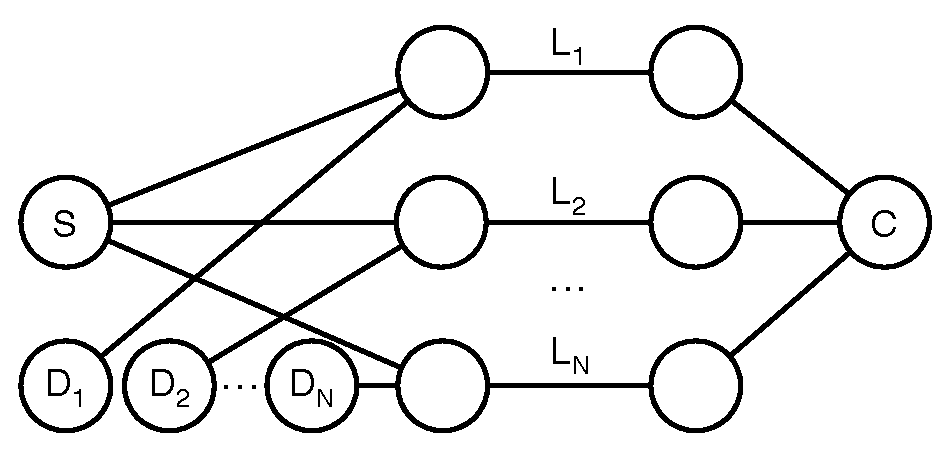
\includegraphics[width=2.5in]{figures/cate/topo}
    \caption{Simulation topology}
    \label{fig:topo}
\end{figure}

Across simulations, as the number of paths increases, total bandwidth $B$ and the number of simultaneous requests $G$ is fixed, providing insight into how efficiently \ac{PREFLEX} balances traffic as the granularity with which it can split traffic becomes coarser.

In order to evaluate how \ac{PREFLEX} shifts traffic in response to loss, additional ``dummy" servers $D_i$ are connected to $C$ through bottleneck link $L_i$.
The simulation runs for time $T$ and is partitioned into $N+2$ intervals starting on $s_i$, in which $s_0$ and $s_{N+1}$ have no traffic to $D_i$. 
Starting at time $s_i$, client $C$ generates $g_i$ requests to $D_i$ according to the same distribution as used to server $S$. 
All requests to $D_i$ end at time $s_{N+1}$. 
Equation \eqref{eq:si} sets the start time $s_i$ for requests to $D_i$ as a function of total simulation time $T$ and number of paths $N$. 
Likewise, equation \eqref{eq:gi} sets the number of simultaneous requests $g_i$ to $D_i$ as a function of $G$, the total number of requests to $S$, and $N$.
\begin{equation}
s_i = T\frac{i}{N+2}
\label{eq:si}
\end{equation}
\begin{equation}
\theta_i = \frac{\frac{1}{N+1-i}}{\sum{\frac{1}{N+1-i}}},  g_i = G\theta_i.
\label{eq:gi}
\end{equation}

Figure \ref{fig:demand} illustrates the number of simultaneous gets from $C$ to $D_i$ for $N=2$ (used in the example shown in figure \ref{fig:two}) and $N=4$. 
Generating cross-traffic in this manner serves two purposes. 
Firstly, $\sum{g_i}=G$, so independently of the number of concurrent paths, the maximum load in the system is $2G$. 
However, as the number of paths increases, the fluctuation in load for each path becomes smaller, stressing the sensitivity with which \ac{PREFLEX} must balance traffic. 
Secondly, the number of requests for each $D_i$ over time is the same. 
Over timescale $T$, equalisation appears to be an acceptable strategy but will however be shown to fail to make efficient use of available capacity. 
This is a fundamental limitation of offline traffic engineering, which is calculated over very long timescales and is unable to adapt as traffic routinely shifts.

\begin{figure}
    \begin{subfigure}[b]{.5\linewidth}
        \centering
        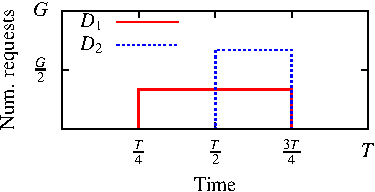
\includegraphics[width=2.25in]{figures/cate/dummy2-crop.pdf}
        \caption{$N=2$}\label{fig:1a}
    \end{subfigure}%
    \begin{subfigure}[b]{.5\linewidth}
        \centering
        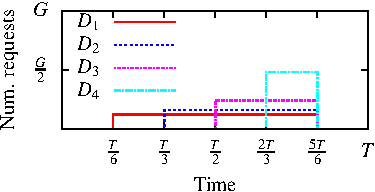
\includegraphics[width=2.25in]{figures/cate/dummy4-crop.pdf}
        \caption{$N=4$}\label{fig:1b}
    \end{subfigure}
    \caption[Number of requests to cross traffic servers.]{Number of requests from $C$ to cross traffic servers $D_i$ for different values of $N$}
    \label{fig:demand}
\end{figure}

The settings used for all simulations, including those previously shown in figure \ref{fig:two}, are as follows.
Total simulation time $T$ is set to $1200$ seconds, while total bandwidth $B$ is fixed at $240$Mbps. 
The number of requests $G$ sent from $C$ to $S$ is set to 240. 
Upon completing, a request is respawned after an idle period following an exponential distribution with a $15$s mean. 
Transfer size follows a Weibull distribution with an average value of $2$MB. 
While artificial, these values attempt to represent traffic to a single prefix with a file size that mimics the small but bursty nature of web traffic, which does not lend itself to being balanced by the end-host. 
\ac{PREFLEX} is configured with $\beta_E = 0.05$, $\mu_{min}=0.01/N$ and $\delta=0.005$.

\subsection{Varying bottleneck distribution}

For the remainder of this section, congestion balancing using \ac{PREFLEX} will be directly compared to equalisation, which mimics existing traffic engineering techniques based on hashing flow tuples for path assignment.
A useful reference point in interpreting results is to examine the case where all bottlenecks share the same bandwidth, $L_i=B/N$.
Under such conditions, figure \ref{fig:goodputeq} shows the goodput, calculated as the total data transfered to client $C$ by flows completed within $T$, as a proportion of total link bandwidth.
The bulk of goodput originates from server $S$, which is the only multi-homed domain.
If traffic is correctly balanced, servers $D_{1-N}$ should generate the same amount of goodput.
While both equalisation and congestion balancing saturate most available bandwidth, the former leads to disproportionate distribution of goodput amongst competing traffic. 
As loss is not equalised over all paths, the amount of goodput achieved by servers $D_i$ differs despite demand being similar.
\begin{figure}
    \centering
    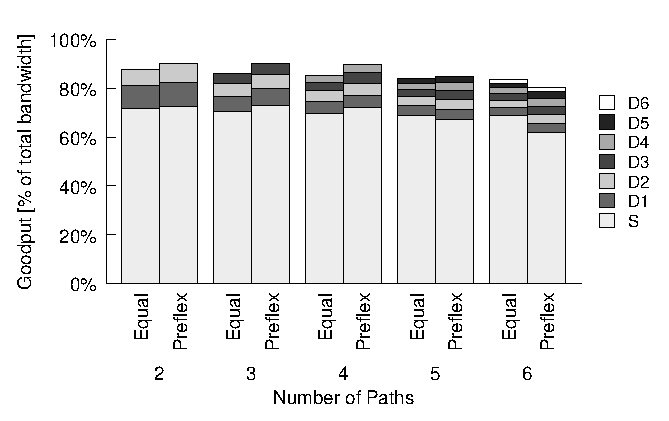
\includegraphics[width=4in]{figures/cate/eqbw}
    \caption[Goodput achieved over equal capacity links.]{Goodput relative to $B$ achieved by each server over equal capacity links.}
    \label{fig:goodputeq}
\end{figure}

In this scenario, equalisation can be seen as the optimal static TE solution, yet both approaches bear similar performance. 
With no knowledge of topology, link bandwidth or expected traffic matrices, \ac{PREFLEX} is able to adequately mimic the performance of the static TE solution for the case where such an approach is best suited.

\begin{figure}
    \centering
    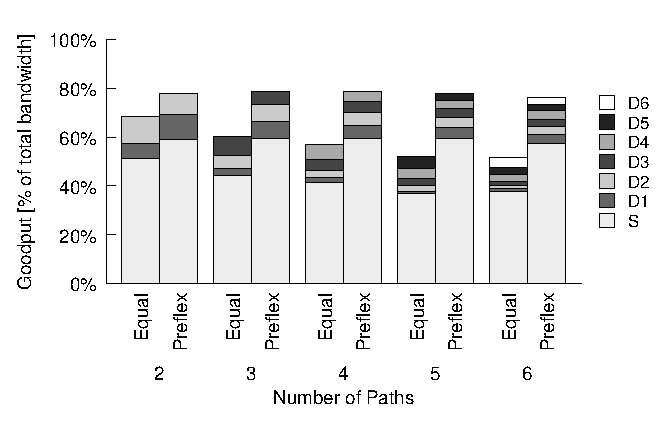
\includegraphics[width=4in]{figures/cate/diffbw}
    \caption[Goodput achieved over unequal capacity links.]{Goodput relative to $B$ achieved by each server over unequal capacity links.}
    \label{fig:goodputdiff}
\end{figure}

Where bottleneck bandwidth is unequal however equalisation is shown to be severely lacking.
The effect of differing bottlenecks is investigated by repeating previous simulations with the same total bandwidth $B$, but with $L_i$ set proportionally to $B$ in a similar manner to \eqref{eq:gi}, that is $L_i = \theta_i B$.
The ensuing results, shown in figure \ref{fig:goodputdiff}, highlight two significant shortcomings of equalisation which \ac{PREFLEX} overcomes. 
Firstly, goodput for $S$ drops as $N$ increases. 
Unable to realize it is overloading a path, equalisation is reduced to sending traffic over each link at approximately the same rate as the most congested link. 
In contrast, \ac{PREFLEX} detects congestion and adapts accordingly. 
Secondly, the incorrect distribution of traffic due to equalisation in $S$ distorts the goodput of competing traffic. 
While in \ac{PREFLEX} goodput from $D_{1-N}$ is perfectly balanced, with equalisation traffic crossing the most congested links are directly affected by another domain's inability to distribute traffic appropriately.
It may seem unfair to judge equalisation for cases where there is a mismatch in link capacity.
However, such a mismatch between link weight and path capacity arises regularly as operators adjust traffic engineering according to local conditions, with little thought spared for the impact this may have further downstream.

\begin{figure}
    \centering
    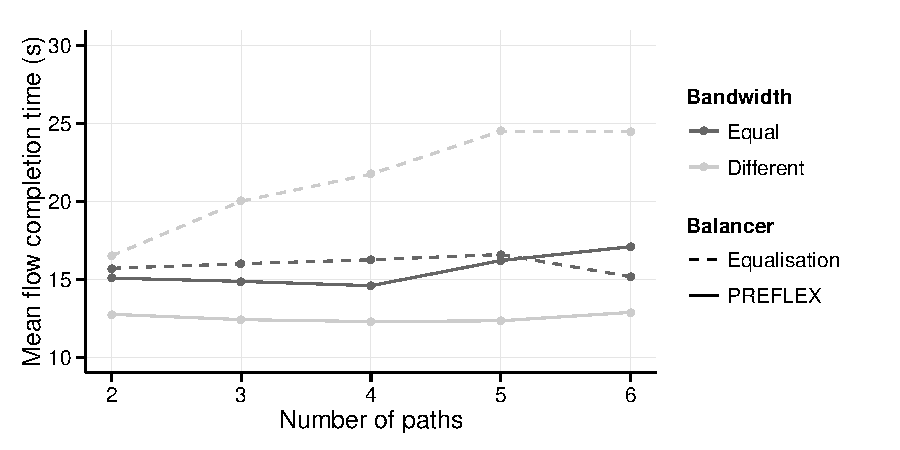
\includegraphics[width=3.2in]{figures/cate/duration}
    \caption[Mean flow completion time.]{Mean flow completion time for equal and differing bottleneck links.}
    \label{fig:duration}
\end{figure}

This impact is in turn perceived by users, who experience longer flow completion times, as shown in figure \ref{fig:duration}. 
In the equal bandwidth case the flow completion time is similar for both balancers.  
Where bandwidth differs however, balancing by congestion outperforms equalisation and maintains a stable performance even for all six paths.  
This shows that the algorithm scales well as the number of available paths increases. 
